%%% ====================================================================
%%%  @LaTeX-file{
%%%     filename        = "dad-user-guide.tex",
%%%     version         = "1.2",
%%%     date            = "2017/05/20",
%%%     author          = "Yannis Haralambous",
%%%     copyright       = "This file is part of the dad package, released
%%%                        under the LPPL."
%%%     keywords        = "TeX, file header,
%%%     supported       = "yes",
%%%     abstract        = "This is the user's guide of the dad
%%%       system for typesetting in the Arabic language.",
%%%  }
%%% ====================================================================
% needs lualatex to be processed
\documentclass[11pt,a4paper]{article}
\usepackage{luatex85}
\pdfmapfile{/hom/yannis/projets/smf/0/smfpdftex.map}
\usepackage{graphicx,color,framed,a4wide}
\usepackage{ifpdf}
%\usepackage[utf8]{inputenc}
\ifpdf
\usepackage[breaklinks,hidelinks]{hyperref}
\usepackage{tikz}
\usetikzlibrary{arrows}
\else 
\usepackage{url}
\fi
\usepackage[colorinlistoftodos]{todonotes}
\usepackage{dad}
\def\hamza{'}%\textsuperscript{\ejective}}
\def\ayn{`}%\textsuperscript{\reveject}}
\usepackage{fontspec}

%%% Start of metadata %%%

\title{User's Guide of \arab{D} (\emph{\d{d}\=ad}),\\ a Simple Arabic Typesetting System\\ for Mixed Latin/Arabic Alphabet Documents\\[12pt]Version 1.2/2017-05-20}

% repeat info for each author.
\author{Yannis Haralambous\thanks{IMT Atlantique,
UMR~CNRS~6285 Lab-STICC,
Technop\^ole Brest Iroise
CS 83818, 29238~Brest~Cedex~3, France, \url{yannis.haralambous@imt-atlantique.fr}}}
%\netaddress{yannis.haralambous (at) telecom-bretagne dot eu}
%\personalURL{http://example.org/~user/}
\date{}
%%% End of metadata %%%


%\newfontfamily\arabicfont[Script=Arabic,Scale=1.2]{Scheherazade-Regular.ttf}
%\newcommand{\textarabic}[1]{\bgroup\textdir TRT\arabicfont #1\egroup}
\begin{document}

\maketitle

\section*{New features of version 1.2}

I added support for Lua\TeX\ 0.95 by including package \verb=luatex85= and by changing \verb=\luatextextdir= into \verb=\textdir=.

\section{Introduction}

\noindent\mbox{\arab{D}} is a package for typesetting Arabic in the simplest possible way. It is particularly well suited for mixed Arabic/Latin documents. ``Simplest possible'' means:
\begin{itemize}
\item it is compatible with all \LaTeX\ style files, since the code is minimal and all the complexity is in the font;
\item input can be done in Unicode or in transliteration, the latter being often the best choice when mixing left-to-right and right-to-left scripts;
\item the only \TeX nical requirement is Lua\TeX, not because of the Lua language (which is not used, for the moment), but because of features that have survived from Lua\TeX's $\Omega$ origins: bidirectionality and use of large fonts (OVF, OFM).
\end{itemize}
Choose Lua\TeX\ as your \TeX\ engine, load the package into your document, and \arab{AhlAaN Us-hlAaN!}, just start writing in Arabic using command \verb=\arab=.

More information about \arab{D} (history, evolution, rationale of technical choices, \TeX nicalities) can be found in \cite{tugboat}.

%\begin{framed}
%\noindent ATTENTION! \textbf{\arab{xTr!}} Because of bugs in Lua\TeX, in some cases appear mysterious blank spaces on the left of the text, word parts are duplicated, and sometimes \TeX\ breaks with an error message \texttt{This can't happen (sub\_disc\_widths).} These errors have been submitted to the Lua\TeX\ team (\url{http://tracker.luatex.org/view.php?id=912&history=1#history}), which will provide the necessary corrections \arab{'in shA| ALLh}.
%\end{framed}

\section{The name}

Thanks to the Internet, search engines, social media, and the like, people are becoming more and more aware of other languages and writing systems. Why not give this package an Arabic name, be it a single letter?

The author has chosen letter \arab{D}, called \emph{\d{d}\=ad}, because Arabic is traditionally called the ``language of the \emph{\d{d}\=ad},'' since this sound was considered as being unique to Arabic.

The reader is probably wondering how to pronounce this letter,technically a ``voiced velarized alveolar stop'' \cite[p.~16]{ryding2014}. Here is how \cite[p.~10]{learn2} describes its pronunciation:

\begin{quotation}
Pronounce the regular sound `d' and you will find that the tip of your tongue will touch in the region of the upper front teeth/gum. Now pronounce the sound again and at the same time depress the \emph{middle} of the tongue. This has the effect of creating a larger space between the tongue and the roof of the mouth and gives the sound produced a distinctive `hollow' characteristic, which also effects the surrounding vowels. It is difficult to find a parallel in English, but the difference between `Sam' and `psalm' (standard English pronunciation) gives a clue. Tense the tongue muscles in pronouncing `psalm' and you are nearly there. Now pronounce the a-vowel of `psalm' before and after `\d{d}', saying `a\d{d}a', keeping the tongue tense, and that's as near as we can get to describing it in print.
\end{quotation}

\section{How to use \arab{D}}

The package provides three PostScript Type~1 fonts (plain,  bold and typewriter), ``real'' fonts (regular TFM) and large virtual fonts (OVF and OFM files). There are also rudimentary FD and STY files, a MAP file, Perl scripts for conversion to (and from) UTF-8, the Perl script which builds the font and finally adjustment files, in case the user wants to change kerning and diacritic placement.

Once the package is installed, to use it just call
\begin{verbatim}
\usepackage{dad}
\end{verbatim}

Notice however that it requires Lua\TeX\ (for change of direction and OVF/OFM compliance).

To typeset in Arabic, one uses the command \verb=\arab= (which is ``long'': paragraph changes are allowed in its argument).

Arabic text can be input in transliteration, as described in Table~\ref{trans} or in Unicode UTF-8 (\S\,\ref{unicode}). 

{\tolerance5000 For example, to obtain \arab{AlkitAb} one would write in transliteration \verb=\arab{=\texttt{AlkitAb}\verb=}= or in Unicode \verb=\arab{=\arabtt{AlkitAb}\verb=}=. By writing \verb=\arabtt{=\texttt{AlkitAb}\verb=}= one obtains the typewriter version \arabtt{AlkitAb} (which is less appealing, but fits quite nicely with the Computer Modern Typewriter font).

}

\begin{table*}[t]
\centering{\renewcommand{\arraystretch}{2}

\caption{Transliteration of \arab{D} system\label{trans}}
\begin{tabular}{|c|c||c|c||c|c||c|c||c|c||c|c|}
\hline
\arab{|}&\texttt{|}&\arab{'A}&\texttt{'A}&\arab{'a}&\texttt{'a}&\arab{'u}&\texttt{'u}&\arab{'i}&\texttt{'i}&\arab{'I}&\texttt{'I}\\
\arab{A}&\texttt{A}&\arab{b}&\texttt{b}&\arab{t*}&\texttt{t*}&\arab{t}&\texttt{t}&\arab{th}&\texttt{th}&\arab{j}&\texttt{j}\\
\arab{H}&\texttt{H}&\arab{x}&\texttt{x}&\arab{d}&\texttt{d}&\arab{dh}&\texttt{dh}&\arab{r}&\texttt{r}&\arab{z}&\texttt{z}\\
\arab{s}&\texttt{s}&\arab{sh}&\texttt{sh}&\arab{S}&\texttt{S}&\arab{D}&\texttt{D}&\arab{T}&\texttt{T}&\arab{Z}&\texttt{Z}\\
\arab{`}&\texttt{`}&\arab{R}&\texttt{R}&\arab{f}&\texttt{f}&\arab{q}&\texttt{q}&\arab{k}&\texttt{k}&\arab{l}&\texttt{l}\\
\arab{m}&\texttt{m}&\arab{n}&\texttt{n}&\arab{h}&\texttt{h}&\arab{U}&\texttt{U}&\arab{I}&\texttt{I}&\arab{Y}&\texttt{Y}\\\hline
\arab{A*}&\texttt{A*}&\arab{^^^^00fbo}&\texttt{o}&\arab{^^^^00fba}&\texttt{a}&\arab{^^^^00fbi}&\texttt{i}&\arab{^^^^00fbu}&\texttt{u}&\arab{^^^^00fbaN}&\texttt{aN}\\
\arab{^^^^00fbiN}&\texttt{iN}&\arab{^^^^00fbuN}&\texttt{uN}&\arab{^^^^00fb+}&\texttt{+}&\arab{^^^^00fb+a}&\texttt{+a}&\arab{^^^^00fb+i}&\texttt{+i}&\arab{^^^^00fb+u}&\texttt{+u}\\
\arab{^^^^00fb+aN}&\texttt{+aN}&\arab{^^^^00fb+iN}&\texttt{+iN}&\arab{^^^^00fb+uN}&\texttt{+uN}&\arab{^^^^00fba*}&\texttt{a*}&\arab{^^^^00fb+a*}&\texttt{+a*}&\arab{LLh}&\texttt{LLh}\\\hline
\arab{p}&\texttt{p}&\arab{g}&\texttt{g}&\arab{C}&\texttt{C}&\arab{J}&\texttt{J}&\arab{e}&\texttt{e}&\arab{v}&\texttt{v}\\\hline
\arab{'b}&\texttt{'b}&\arab{'n}&\texttt{'n}&\arab{'f}&\texttt{'f}&\arab{'q}&\texttt{'q}&\arab{^^^^00fba**}&\texttt{a**}&\arab{^^^^00fb+a**}&\texttt{+a**}\\\hline
\end{tabular}

}
\end{table*}

\clubpenalty10000

\subsection{Rationale of the transliteration}

Here are the rules of the proposed transliteration: 
\begin{enumerate}
\item pharyngeal \arabttexample{H}, emphatic \arabttexample{S}, \arabttexample{D}, \arabttexample{T},
\arabttexample{Z} and velar \arabttexample{R} are \emph{uppercased}---do not confuse them with glottal \arabttexample{h}, non-emphatic \arabttexample{s}, \arabttexample{d}, \arabttexample{t}, \arabttexample{z}, and alveolar \arabttexample{r};
\item long vowels (\arabttexample{A}, \arabttexample{U}, \arabttexample{Y}) and
\emph{\hamza$\!$alif maq\d s\=ura} (\arabttexample{I}) are also
\emph{uppercased};

\item some consonants are modified by adding a character \texttt{h} (\arabttexample{dh}, \arabttexample{th}, \arabttexample{sh});

\item the stand-alone \emph{hamza} is obtained by a vertical bar \texttt{|} and letter ayn by a grave accent (which, in legacy \TeX\ produces an inverted curly apostrophe, which is sometimes used to transliterate this letter);

\item to avoid confusion between pairs of letters and letters obtained by digraphs, one has to use a dash to separate characters: compare \arabttexample{s-h} and \arabttexample{sh}, or \arabttexample{t-h} and \arabttexample{th};

\item more generally, the dash plays the r\^ole of \emph{zero-width joiner}\footnote{Except for the case of letter \arabttexample{dh} which is biform and hence is not connected with the following letter. By writing \arabttexample{d-h} one obtains letters \emph{d\=al} and \emph{h\=a\hamza}, but the \emph{h\=a\hamza} is not in medial form, as it would be in any other case when preceded by a dash.}: when writing \arabttexample{-b}, the letter \emph{b\=a\hamza} will be in final form; \arabttexample{b-} and \arabttexample{-b-} will produce initial and middle letters, provided of course the letter is quadriform (as is letter \emph{b\=a\hamza} in this example). This is very useful when describing grammar rules, to signify that a letter (or letter group) is an affix;

\item the dash can also be used to reestablish contextual forms when combined with \TeX\ commands, for example, to colorize letters. There is only one special case: when we want to colorize a letter of an isolated ligature \arab{lA}, instead of a dash, we use digit \texttt{4}. For the final ligature \arab{-lA} it will be a digit \texttt{5}. Example: to colorize the \emph{l\=am}s of \arab{t-\textcolor{red}{-l5-}-A5\textcolor{red}{l4-}-A4}, write
\begin{verbatim}
\arab{t-\textcolor{red}{-l5-}-A5%
\textcolor{red}{l4-}-A4}
\end{verbatim}

%\def\kesh{\leavevmode\leaders\hrule height\fontdimen8\hfill\kern0pt}

\item finally, there is yet another use of the dash: when doubled, it produces a kashida
%tatweel
%(also known as ``kashida'') 
stroke: compare \arabttexample{lYl} and \arabttexample{l--Y--l}. There is also a \verb=\kesh= command for extensible kashida (it is equivalent to a \verb=\hrulefill= using the default rule thickness font dimension \verb=\fontdimen8=): \verb=l--\kesh--Y--\kesh--l.= will produce:

\noindent\arab{l--\kesh--Y--\kesh--l.}

\item some digraphs start with an apostrophe: it is the case of \emph{hamza}-carriers \arabttexample{'a}, \arabttexample{'i}, \arabttexample{'u}, \arabttexample{'I}, \arabttexample{'A} but also of undotted letters \emph{b\=a\hamza} \arabttexample{'b}, \emph{n\=un} \arabttexample{'n}, \emph{f\=a\hamza} \arabttexample{'f} and \emph{q\=af} \arabttexample{'q};

\item other digraphs end with one or more asterisks: the most frequent one is the \emph{t\=a\hamza\ marbu\d{t}a} \arabttexample{t*} (which can be used also in initial and medial, and then becomes a regular \emph{t\=a\hamza}). The asterisk is also used for the \emph{Ua\d{s}la} (which is only placed on the \emph{\hamza$\!$alif}) \arabttexample{A*} as well as for the vertical \emph{fat\d{h}a} (as in \arabttexample{ha*dhA}) and the \emph{madda}. The latter is normally used only on the \emph{\hamza$\!$alif} (\arabttexample{'A}) but can be found also in the notorious \emph{muqa\d t\d ta\ayn\=at} in the Koran, as in \arab{`a**sa**qa**} (\emph{Koran} 42:2) or \arab{ka**ha*Ya*`a**Sa**} (\emph{Koran} 19:1)---sometimes it is even combined with a \emph{\v{s}adda} (as in \arab{Ala**m+a**Sa**}, \emph{Koran} 7:1 and \cite[p.~111]{syed} for the \emph{\v{s}adda});

\item there is a special transcription for the ligature \arabttexample{LLh} used for the \arab{اسم الجلالة} ``noun of majesty,'' which is the name of God \arab{ALLh}: in this case---and in this case only---an uppercase \texttt{L} is used. The reason is that we wish to avoid ambiguity with other uses of the trigram \emph{l\=am}-\emph{l\=am}-\emph{h\=a\hamza}, for example \arab{YuDolilohu} (\emph{Koran} 6:39) where we encounter letters \arab{llh} but not with the meaning ``God.'' Contrarily to other systems, the \arab{LLh} ligature is available also in final form (for \arab{faLiLhi} which occurs six times in the Koran, for example  \emph{Koran} 6:149), and it is possible to add diacritics to its first glyph (as in \arab{UaLiLhi}, \emph{Koran} 2:115 or \arab{L+iLhi}, \emph{Koran} 2:165).
\end{enumerate}

\begin{figure*}[p]
\arab{\begin{center}
\textbf{rbA`YAt AlxYAm}

\medskip

\begin{minipage}{10cm}
sm`t SUtA hAtfA fY AlsH--\kesh--r n--\kesh--AdI mn AlRYb rfAt Albsh--\kesh--r\\
hbUA Aml'aUA k'as AlmnI qb--\kesh--l 'an tml'a k--\kesh--'as Al`m--\kesh--r kf Alq--\kesh--dr\\
lA tshRl AlbAl bmADY Alzm--\kesh--An UlA b--\kesh--'At Al`Y--\kesh--sh qb--\kesh--l Al'aUAn\\
U'aR--\kesh--nm mn AlHAD--\kesh--r ldhAt--\kesh--h flYs f--\kesh--Y Tb--\kesh--` AllYAl--\kesh--Y Al'am--\kesh--An\\
Rd bZhr AlRYb UAlYUm l--\kesh--Y Ukm YxYb AlZ--\kesh--n f--\kesh--Y Almqb--\kesh--l\\
Uls--\kesh--t bAlRAf--\kesh--l Ht--\kesh--I 'arI jm--\kesh--Al dnY--\kesh--AY U lA Ajtl--\kesh--I\\
Alqlb qd 'aDnAh `shq Aljm--\kesh--Al UAlS--\kesh--dr q--\kesh--d D--\kesh--Aq bm--\kesh--A lA Yq--\kesh--Al\\
YA rb hl YrDYk hdhA AlZlm--\kesh--A UAlm--\kesh--A| Yns--\kesh--Ab 'am--\kesh--Am--\kesh--Y zlAl\\
'aUlI bhdhA Alqlb 'an Yxfq--\kesh--A U fY RrAm AlH--\kesh--b 'an YHtrq--\kesh--A\\
mA 'aDY` AlYUm AldhY m--\kesh--r b--\kesh--Y mn RYr 'an 'ahUI U 'an 'a`shq--\kesh--A\\
'afq xfYf AlZl hdhA AlsH--\kesh--r n--\kesh--AdI d` Aln--\kesh--Um Un--\kesh--AR AlUt--\kesh--r\\
fm--\kesh--A 'aT--\kesh--Al Aln--\kesh--Um `m--\kesh--rA UlA qSr mn Al'a`mAr TUl Als-h--\kesh--r\\
fk--\kesh--m tUl--\kesh--I AllY--\kesh--l b`--\kesh--d Alnh--\kesh--Ar UT--\kesh--Al bAl'anj--\kesh--m h--\kesh--dhA Alm--\kesh--dAr\\
f'amsh AlhUYnt* 'an hdhA Alc--\kesh--rI m--\kesh--n 'a`Y--\kesh--n sAH--\kesh--rt* AlAH--\kesh--UrAr\\
lA tUHsh Alnfs bxUf AlZn--\kesh--Un U'aRnm mn AlHADr 'amn AlYqY--\kesh--n\\
fqd tsAUI fY AlcrI rAH--\kesh--l RdA UmAD mn AlUf AlsnY--\kesh--n\\
ATf'I lZI Alqlb bshhd AlrD--\kesh--Ab f'inm--\kesh--A Al'aY--\kesh--Am mc--\kesh--l AlsH--\kesh--Ab\\
U`Yshn--\kesh--A TY--\kesh--f xY--\kesh--Al fn--\kesh--l HZ--\kesh--k mn--\kesh--h qb--\kesh--l f--\kesh--Ut Alshb--\kesh--Ab\\
lbst cUb Al`Ysh lm Astsh--\kesh--r UH--\kesh--rt fY--\kesh--h bY--\kesh--n sht--\kesh--I Alfk--\kesh--r\\
UsUf 'anDU AlcUb `nY Ul--\kesh--m 'adrk lm--\kesh--AdhA j'I--\kesh--t 'aY--\kesh--n AlmR--\kesh--r\\
YA mn YHAr Alfhm fY qdrt--\kesh--k UtTl--\kesh--b Alnf--\kesh--s Hm--\kesh--I TA`t--\kesh--k\\
Askrn--\kesh--Y Al'ic--\kesh--m U lknn--\kesh--Y SH--\kesh--Ut bAl'am--\kesh--Al f--\kesh--Y rHmt--\kesh--k\\
'in lm 'akn 'axlSt fY TA`t--\kesh--k f'inn--\kesh--Y 'aTm--\kesh--` f--\kesh--Y rHmt--\kesh--k\\
U'inm--\kesh--A Yshf--\kesh--` l--\kesh--Y b'ann--\kesh--Y q--\kesh--d `sh--\kesh--t lA 'ash--\kesh--rk fY UHdt--\kesh--k\\
nxfY `n AlnAs snI Tl`t--\kesh--k f'inn--\kesh--Y 'aTm--\kesh--` f--\kesh--Y rHmt--\kesh--k\\
f'an--\kesh--t mj--\kesh--lAh U'an--\kesh--t Al--\kesh--dhY t--\kesh--rI bdY--\kesh--` AlSn--\kesh--` f--\kesh--Y 'AYt--\kesh--k\\
An tfDl AlqTrt* mn bHrh--\kesh--A ff--\kesh--Y m--\kesh--dAh--\kesh--A mnt-h--\kesh--I 'amrh--\kesh--A\\
tqArb--\kesh--t Y--\kesh--A rb m--\kesh--A bYnn--\kesh--A msAf--\kesh--t* Alb`--\kesh--d `l--\kesh--I qdrh--\kesh--A\\
YA `Alm Al'asrAr `lm AlYq--\kesh--Y--\kesh--n Y--\kesh--A kAsh--\kesh--f AlD--\kesh--r `--\kesh--n AlbA'IsY--\kesh--n\\
Y--\kesh--A qAb--\kesh--l Al'a`--\kesh--dhAr `dn--\kesh--A 'il--\kesh--I Zl--\kesh--k f'aqb--\kesh--l tUb--\kesh--t* AltA'IbY--\kesh--n
\end{minipage}
\end{center}}
\caption{The lyrics of the song \arab{rbA`YAt AlxYAm} (Oum Kalthoum, 1950) \cite{oum}\label{oum}}
\end{figure*}

\begin{figure*}[p]

\kern-2cm

\scriptsize
\begin{verbatim}
\documentclass{article}
\usepackage{dad}
\begin{document}
\arab{
\begin{center}
\textbf{rbA`YAt AlxYAm}

\medskip

\begin{minipage}{10cm}
sm`t SUtA hAtfA fY AlsH--\kesh--r n--\kesh--AdI mn AlRYb rfAt Albsh--\kesh--r\\
hbUA Aml'aUA k'as AlmnI qb--\kesh--l 'an tml'a k--\kesh--'as Al`m--\kesh--r kf
Alq--\kesh--dr\\
lA tshRl AlbAl bmADY Alzm--\kesh--An UlA b--\kesh--'At Al`Y--\kesh--sh qb--\kesh--l
Al'aUAn\\
U'aR--\kesh--nm mn AlHAD--\kesh--r ldhAt--\kesh--h flYs f--\kesh--Y Tb--\kesh--`
AllYAl--\kesh--Y Al'am--\kesh--An\\
Rd bZhr AlRYb UAlYUm l--\kesh--Y Ukm YxYb AlZ--\kesh--n f--\kesh--Y Almqb--\kesh--l\\
Uls--\kesh--t bAlRAf--\kesh--l Ht--\kesh--I 'arI jm--\kesh--Al dnY--\kesh--AY U
lA Ajtl--\kesh--I\\
Alqlb qd 'aDnAh `shq Aljm--\kesh--Al UAlS--\kesh--dr q--\kesh--d D--\kesh--Aq bm--\kesh--A
lA Yq--\kesh--Al\\
YA rb hl YrDYk hdhA AlZlm--\kesh--A UAlm--\kesh--A| Yns--\kesh--Ab 'am--\kesh--Am--\kesh--Y
zlAl\\
'aUlI bhdhA Alqlb 'an Yxfq--\kesh--A U fY RrAm AlH--\kesh--b 'an YHtrq--\kesh--A\\
mA 'aDY` AlYUm AldhY m--\kesh--r b--\kesh--Y mn RYr 'an 'ahUI U 'an 'a`shq--\kesh--A\\
'afq xfYf AlZl hdhA AlsH--\kesh--r n--\kesh--AdI d` Aln--\kesh--Um Un--\kesh--AR
AlUt--\kesh--r\\
fm--\kesh--A 'aT--\kesh--Al Aln--\kesh--Um `m--\kesh--rA UlA qSr mn Al'a`mAr TUl
Als-h--\kesh--r\\
fk--\kesh--m tUl--\kesh--I AllY--\kesh--l b`--\kesh--d Alnh--\kesh--Ar UT--\kesh--Al
bAl'anj--\kesh--m h--\kesh--dhA Alm--\kesh--dAr\\
f'amsh AlhUYnt* 'an hdhA Alc--\kesh--rI m--\kesh--n 'a`Y--\kesh--n sAH--\kesh--rt*
AlAH--\kesh--UrAr\\
lA tUHsh Alnfs bxUf AlZn--\kesh--Un U'aRnm mn AlHADr 'amn AlYqY--\kesh--n\\
fqd tsAUI fY AlcrI rAH--\kesh--l RdA UmAD mn AlUf AlsnY--\kesh--n\\
ATf'I lZI Alqlb bshhd AlrD--\kesh--Ab f'inm--\kesh--A Al'aY--\kesh--Am mc--\kesh--l
AlsH--\kesh--Ab\\
U`Yshn--\kesh--A TY--\kesh--f xY--\kesh--Al fn--\kesh--l HZ--\kesh--k mn--\kesh--h
qb--\kesh--l f--\kesh--Ut Alshb--\kesh--Ab\\
lbst cUb Al`Ysh lm Astsh--\kesh--r UH--\kesh--rt fY--\kesh--h bY--\kesh--n sht--\kesh--I
Alfk--\kesh--r\\
UsUf 'anDU AlcUb `nY Ul--\kesh--m 'adrk lm--\kesh--AdhA j'I--\kesh--t 'aY--\kesh--n
AlmR--\kesh--r\\
YA mn YHAr Alfhm fY qdrt--\kesh--k UtTl--\kesh--b Alnf--\kesh--s Hm--\kesh--I TA`t--\kesh--k\\
Askrn--\kesh--Y Al'ic--\kesh--m U lknn--\kesh--Y SH--\kesh--Ut bAl'am--\kesh--Al
f--\kesh--Y rHmt--\kesh--k\\
'in lm 'akn 'axlSt fY TA`t--\kesh--k f'inn--\kesh--Y 'aTm--\kesh--` f--\kesh--Y
rHmt--\kesh--k\\
U'inm--\kesh--A Yshf--\kesh--` l--\kesh--Y b'ann--\kesh--Y q--\kesh--d `sh--\kesh--t
lA 'ash--\kesh--rk fY UHdt--\kesh--k\\
nxfY `n AlnAs snI Tl`t--\kesh--k f'inn--\kesh--Y 'aTm--\kesh--` f--\kesh--Y rHmt--\kesh--k\\
f'an--\kesh--t mj--\kesh--lAh U'an--\kesh--t Al--\kesh--dhY t--\kesh--rI bdY--\kesh--`
AlSn--\kesh--` f--\kesh--Y 'AYt--\kesh--k\\
An tfDl AlqTrt* mn bHrh--\kesh--A ff--\kesh--Y m--\kesh--dAh--\kesh--A mnt-h--\kesh--I
'amrh--\kesh--A\\
tqArb--\kesh--t Y--\kesh--A rb m--\kesh--A bYnn--\kesh--A msAf--\kesh--t* Alb`--\kesh--d
`l--\kesh--I qdrh--\kesh--A\\
YA `Alm Al'asrAr `lm AlYq--\kesh--Y--\kesh--n Y--\kesh--A kAsh--\kesh--f AlD--\kesh--r
`--\kesh--n AlbA'IsY--\kesh--n\\
Y--\kesh--A qAb--\kesh--l Al'a`--\kesh--dhAr `dn--\kesh--A 'il--\kesh--I Zl--\kesh--k
f'aqb--\kesh--l tUb--\kesh--t* AltA'IbY--\kesh--n
\end{minipage}
\end{center}
}
\end{document}
\end{verbatim}
\caption{\TeX\ code of Fig.~\ref{oum}, transliterated input}
\end{figure*}

\begin{figure*}[p]

\kern-2cm

\scriptsize
\begin{verbatim}
\documentclass{article}
\usepackage{dad}
\begin{document}
\arab{
\begin{center}
\end{verbatim}

\kern-1.2\baselineskip

\verb=\textbf{=\arabtt{rbA`YAt AlxYAm}\verb=}=

\kern-1.2\baselineskip

\begin{verbatim}

\medskip

\begin{minipage}{10cm}
\end{verbatim}
\def\CRCRCR{\textbackslash\textbackslash\\}
\arabtt{sm`t SUtA hAtfA fY AlsH--\textbackslash tT --r n--\textbackslash tT --AdI mn AlRYb rfAt Albsh--\textbackslash tT --r\CRCRCR
hbUA Aml'aUA k'as AlmnI qb--\textbackslash tT --l 'an tml'a k--\textbackslash tT --'as Al`m--\textbackslash tT --r kf
Alq--\textbackslash tT --dr\CRCRCR
lA tshRl AlbAl bmADY Alzm--\textbackslash tT --An UlA b--\textbackslash tT --'At Al`Y--\textbackslash tT --sh qb--\textbackslash tT --l
Al'aUAn\CRCRCR
U'aR--\textbackslash tT --nm mn AlHAD--\textbackslash tT --r ldhAt--\textbackslash tT --h flYs f--\textbackslash tT --Y Tb--\textbackslash tT --`
AllYAl--\textbackslash tT --Y Al'am--\textbackslash tT --An\CRCRCR
Rd bZhr AlRYb UAlYUm l--\textbackslash tT --Y Ukm YxYb AlZ--\textbackslash tT --n f--\textbackslash tT --Y Almqb--\textbackslash tT --l\CRCRCR
Uls--\textbackslash tT --t bAlRAf--\textbackslash tT --l Ht--\textbackslash tT --I 'arI jm--\textbackslash tT --Al dnY--\textbackslash tT --AY U
lA Ajtl--\textbackslash tT --I\CRCRCR
Alqlb qd 'aDnAh `shq Aljm--\textbackslash tT --Al UAlS--\textbackslash tT --dr q--\textbackslash tT --d D--\textbackslash tT --Aq bm--\textbackslash tT --A
lA Yq--\textbackslash tT --Al\CRCRCR
YA rb hl YrDYk hdhA AlZlm--\textbackslash tT --A UAlm--\textbackslash tT --A| Yns--\textbackslash tT --Ab 'am--\textbackslash tT --Am--\textbackslash tT --Y
zlAl\CRCRCR
'aUlI bhdhA Alqlb 'an Yxfq--\textbackslash tT --A U fY RrAm AlH--\textbackslash tT --b 'an YHtrq--\textbackslash tT --A\CRCRCR
mA 'aDY` AlYUm AldhY m--\textbackslash tT --r b--\textbackslash tT --Y mn RYr 'an 'ahUI U 'an 'a`shq--\textbackslash tT --A\CRCRCR
'afq xfYf AlZl hdhA AlsH--\textbackslash tT --r n--\textbackslash tT --AdI d` Aln--\textbackslash tT --Um Un--\textbackslash tT --AR\\
AlUt--\textbackslash tT --r\CRCRCR
fm--\textbackslash tT --A 'aT--\textbackslash tT --Al Aln--\textbackslash tT --Um `m--\textbackslash tT --rA UlA qSr mn Al'a`mAr TUl
Als-h--\textbackslash tT --r\CRCRCR
fk--\textbackslash tT --m tUl--\textbackslash tT --I AllY--\textbackslash tT --l b`--\textbackslash tT --d Alnh--\textbackslash tT --Ar UT--\textbackslash tT --Al
bAl'anj--\textbackslash tT --m h--\textbackslash tT --dhA Alm--\textbackslash tT --dAr\CRCRCR
f'amsh AlhUYnt* 'an hdhA Alc--\textbackslash tT --rI m--\textbackslash tT --n 'a`Y--\textbackslash tT --n sAH--\textbackslash tT --rt*
AlAH--\textbackslash tT --UrAr\CRCRCR
lA tUHsh Alnfs bxUf AlZn--\textbackslash tT --Un U'aRnm mn AlHADr 'amn AlYqY--\textbackslash tT --n\CRCRCR
fqd tsAUI fY AlcrI rAH--\textbackslash tT --l RdA UmAD mn AlUf AlsnY--\textbackslash tT --n\CRCRCR
ATf'I lZI Alqlb bshhd AlrD--\textbackslash tT --Ab f'inm--\textbackslash tT --A Al'aY--\textbackslash tT --Am mc--\textbackslash tT --l
AlsH--\textbackslash tT --Ab\CRCRCR
U`Yshn--\textbackslash tT --A TY--\textbackslash tT --f xY--\textbackslash tT --Al fn--\textbackslash tT --l HZ--\textbackslash tT --k mn--\textbackslash tT --h
qb--\textbackslash tT --l f--\textbackslash tT --Ut Alshb--\textbackslash tT --Ab\CRCRCR
lbst cUb Al`Ysh lm Astsh--\textbackslash tT --r UH--\textbackslash tT --rt fY--\textbackslash tT --h bY--\textbackslash tT --n sht--\textbackslash tT --I
Alfk--\textbackslash tT --r\CRCRCR
UsUf 'anDU AlcUb `nY Ul--\textbackslash tT --m 'adrk lm--\textbackslash tT --AdhA j'I--\textbackslash tT --t 'aY--\textbackslash tT --n
AlmR--\textbackslash tT --r\CRCRCR
YA mn YHAr Alfhm fY qdrt--\textbackslash tT --k UtTl--\textbackslash tT --b Alnf--\textbackslash tT --s Hm--\textbackslash tT --I TA`t--\textbackslash tT --k\CRCRCR
Askrn--\textbackslash tT --Y Al'ic--\textbackslash tT --m U lknn--\textbackslash tT --Y SH--\textbackslash tT --Ut bAl'am--\textbackslash tT --Al
f--\textbackslash tT --Y rHmt--\textbackslash tT --k\CRCRCR
'in lm 'akn 'axlSt fY TA`t--\textbackslash tT --k f'inn--\textbackslash tT --Y 'aTm--\textbackslash tT --` f--\textbackslash tT --Y
rHmt--\textbackslash tT --k\CRCRCR
U'inm--\textbackslash tT --A Yshf--\textbackslash tT --` l--\textbackslash tT --Y b'ann--\textbackslash tT --Y q--\textbackslash tT --d `sh--\textbackslash tT --t
lA 'ash--\textbackslash tT --rk fY UHdt--\textbackslash tT --k\CRCRCR
nxfY `n AlnAs snI Tl`t--\textbackslash tT --k f'inn--\textbackslash tT --Y 'aTm--\textbackslash tT --` f--\textbackslash tT --Y rHmt--\textbackslash tT --k\CRCRCR
f'an--\textbackslash tT --t mj--\textbackslash tT --lAh U'an--\textbackslash tT --t Al--\textbackslash tT --dhY t--\textbackslash tT --rI bdY--\textbackslash tT --`
AlSn--\textbackslash tT --` f--\textbackslash tT --Y 'AYt--\textbackslash tT --k\CRCRCR
An tfDl AlqTrt* mn bHrh--\textbackslash tT --A ff--\textbackslash tT --Y m--\textbackslash tT --dAh--\textbackslash tT --A mnt-h--\textbackslash tT --I
'amrh--\textbackslash tT --A\CRCRCR
tqArb--\textbackslash tT --t Y--\textbackslash tT --A rb m--\textbackslash tT --A bYnn--\textbackslash tT --A msAf--\textbackslash tT --t* Alb`--\textbackslash tT --d
`l--\textbackslash tT --I qdrh--\textbackslash tT --A\CRCRCR
YA `Alm Al'asrAr `lm AlYq--\textbackslash tT --Y--\textbackslash tT --n Y--\textbackslash tT --A kAsh--\textbackslash tT --f AlD--\textbackslash tT --r
`--\textbackslash tT --n AlbA'IsY--\textbackslash tT --n\CRCRCR
Y--\textbackslash tT --A qAb--\textbackslash tT --l Al'a`--\textbackslash tT --dhAr `dn--\textbackslash tT --A 'il--\textbackslash tT --I Zl--\textbackslash tT --k
f'aqb--\textbackslash tT --l tUb--\textbackslash tT --t*\\
AltA'IbY--\textbackslash tT --n\hfill}
\begin{verbatim}
\end{minipage}
\end{center}
}
\end{document}
\end{verbatim}
\caption{\TeX\ code of Fig.~\ref{oum}, Unicode input}
\end{figure*}

\subsection{Unicode input}\label{unicode}

Input can be transliterated or provided directly in Unicode Arabic: \texttt{\textbackslash arab\{YAnis\}} or \texttt{\textbackslash arab\{\arabtt{YAn--is}\}} or even \texttt{\textbackslash arab\{\arabtt{YA}\,nis\}} or \texttt{\textbackslash arab\{YA\,\arabtt{n--is}\}} will produce the same result: \arab{YAnis}.

All cells of Table~\ref{trans} can be obtained by the corresponding Unicode characters (mostly via a single character, except for \emph{\v{s}adda} + vowel combinations which require two characters). There is a special case, though: the \arab{LLh} ligature (see next section).

For the convenience of the user who wants to write kashida (so that Arabic input is not disrupted) we have defined a command (in Arabic characters) \arabtt{tT}\textbackslash{} (\arab{tT} are the first two letters of \arab{tTUYl} = \emph{ta\d{t}Uyl}, the Arabic name of kashida) which is exactly equivalent to \verb=\kesh= and has to be placed between Unicode \textsc{U+0640 arabic tatwell} characters.

\subsubsection{The \arab{LLh} ligature and Unicode}\label{allah}

The \arab{LLh} ligature is traditionally used for writing the name of God: \arab{ALLh}. It can be found in religious texts, but also in expressions (for example, \arab{'in shA| ALLh} which means ``hopefully'' appears even in French language as \emph{inchallah} and in Portuguese as \emph{oxal\'a}) and in the very common surname \arab{`bd ALLh} Abdallah.

The problem with this ligature is that it contains a rather rare diacritic (a \emph{\v{s}adda} combined with a vertical \emph{fat\d{h}a}---the latter us available on Apple Arabic keyboard layout but not on the Microsoft one) and, as a convenience, most standard fonts will replace the character string \emph{l\=am}-\emph{l\=am}-\emph{h\=a\hamza} (which would normally look like \arab{llh}) by the complete ligature \arab{LLh} (in other words: the font not only changes the glyphs but, at the same time, also adds the diacritics). This behavior is barely legitimate: a ligature (as in `fi' or `\arab{lA}') is normally limited to a change of glyphs, and should not add new characters (in this case, characters \textsc{U+0651 arabic shadda} and \textsc{U+0671 arabic letter superscript alef}) since this means that what is rendered does not correspond anymore to the underlying Unicode character string.

Nevertheless, for the user's convenience, we have adopted that behavior also in \arab{D}, but only in the case of Unicode input. Therefore when the user types Unicode \emph{l\=am}-\emph{l\=am}-\emph{h\=a\hamza} (the first \emph{l\=am} must not be preceded by a quadriform letter), the system will produce the \arab{LLh} ligature.

This method will not work if a diacritic is inserted between the two \emph{l\=am}s, or if the first \emph{l\=am} follows a quadriform letter and hence will be medial. For that case, we have defined a macro \arabtt{llh}\verb=/= (the macro name is in Arabic script so that right-to-left direction is not disrupted) which takes an argument: the vowel between the two \emph{l\=am}s. Hence, to obtain \arab{faLiLhi} the user can choose between one of the following two:
\begin{quote}
\arabtt{^^^^00fbi}\texttt{\{}\arabtt{^^^^00fbi}\texttt{\}}\arabtt{llh}\texttt{/}\arabtt{f--a}\\[6pt]
\texttt{faLiLhi}
\end{quote}
(The dotted circle, used to show the combining nature of short vowels and other diacritics, can be obtained by the macros \verb=\arabdottedcircle= or \arabtt{dA'Irt*}\verb=/= with the macro name in Arabic script.)

\begin{figure*}
{\centering

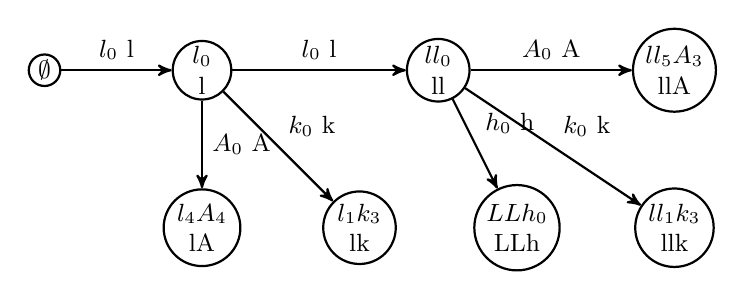
\begin{tikzpicture}[->,>=stealth',x=2cm,y=2cm,auto,node distance=3cm,
  thick,main node/.style={circle,inner sep=1pt,draw,align=center,font=\small}]

\node[main node] (8) at (-1,1)  {$\emptyset$};
\node[main node] (1) at (0,1)  {$l_0$\\\arab{l}};
\node[main node] (2) at (1.5,1)  {$ll_0$\\\arab{ll}};
\node[main node] (3) at (3,1)  {$ll_5A_3$\\\arab{llA}};
\node[main node] (4) at (3,0)  {$ll_1k_3$\\\arab{llk}};
\node[main node] (5) at (2,0)  {$LLh_0$\\\arab{LLh}};
\node[main node] (6) at (1,0) {$l_1k_3$\\\arab{lk}};
\node[main node] (7) at (0,0) {$l_4A_4$\\\arab{lA}};

\path[every node/.style={font=\small}]
(8) edge node {$l_0$ \arab{l}} (1)
(1) edge node {$l_0$ \arab{l}} (2)
(2) edge node {$A_0$ \arab{A}} (3)
(2) edge node {$k_0$ \arab{k}} (4)
(2) edge node {$h_0$ \arab{h}} (5)
(1) edge node {$k_0$ \arab{k}} (6)
(1) edge node {$A_0$ \arab{A}} (7)
;
\end{tikzpicture}

}
\caption{Finite state automaton starting with an isolated \emph{l\=am} (\emph{\hamza$\!$alif} \arab{A} stands for the set of letter $\mathcal{A}={}\{$ \arab{A}, \arab{'a}, \arab{'i}, \arab{'A}, \arab{A*} $\}$; \arab{k} stands for any Arabic letter besides \arab{h} and set $\mathcal{A}$.\label{fsa}}
\end{figure*}

\section{\TeX nicalities}\label{technica}

More information about \arab{D} (history, evolution, rationale of technical choices, \TeX nicalities) can be found in \cite{tugboat}.

\bibliographystyle{plain}  % we recommend the plain bibliography style
\bibliography{dad-user-guide}       % xampl.bib comes with BibTeX

\end{document}